This section motivates the use of dynamic core composition and its impact on performance and energy.
It also shows that loop optimisations have a significant performance impact when fusing cores.
As instructions per cycle (IPC) is a commonly used method of measuring performance, it is used throughout this chapter.

\subsection{Dynamic Core Composition}
\begin{figure}[t]
    \centering
    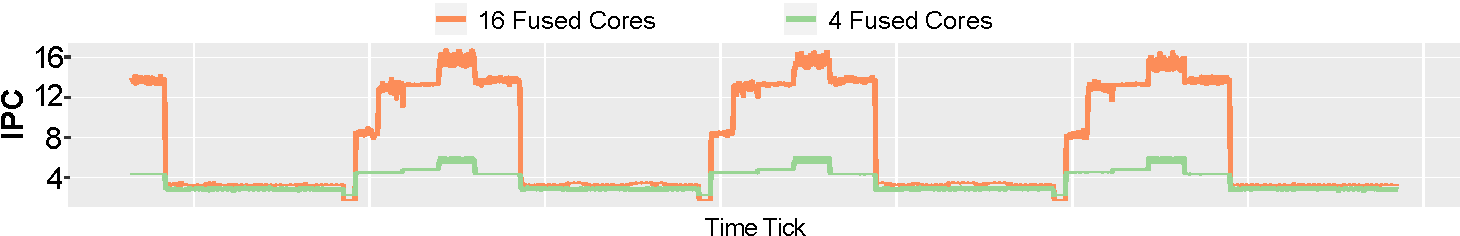
\includegraphics[width=\textwidth]{cases-paper/graphics/motivation/disp_opt_4_16_3.pdf}
    \caption{IPC of a typical benchmark (Disparity from SD-VBS) when executing on a composition of 4 or 16 core processor.} 
    \label{fig:disp_ex}
	\vspace{-2em}
\end{figure}

%\begin{figure}[t]
%    \centering
%    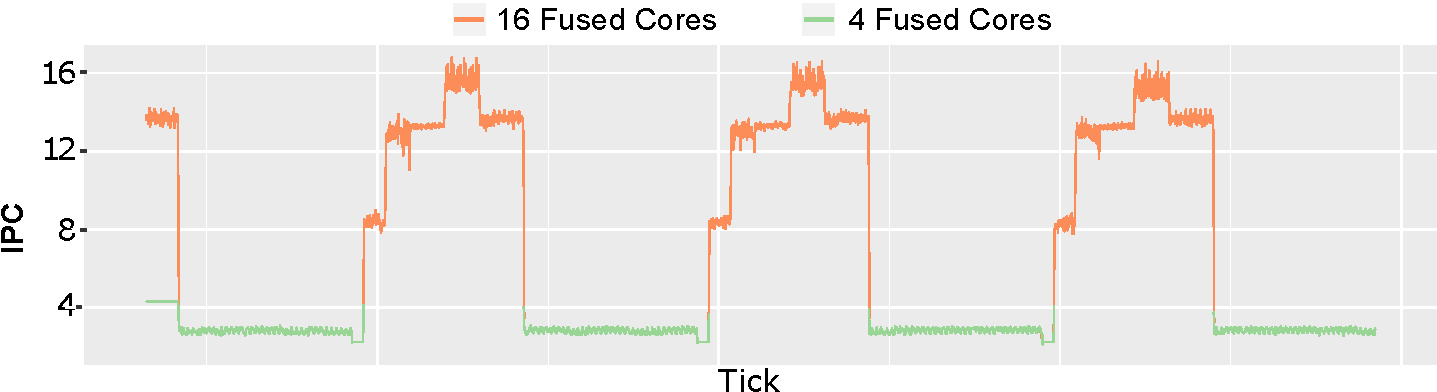
\includegraphics[width=\textwidth]{cases-paper/graphics/motivation/motiv3merge.pdf}
%    \caption{Example of ideal switching between 4 and 16 cores on a DMP for the Disparity benchmark.} 
%    \label{fig:ideal_switch}
%\vspace{2em}
%\end{figure}


\lstset{
	backgroundcolor=\color{lbcolor},
	tabsize=2,
	rulecolor=,
	language=matlab,
        basicstyle=\tiny,
        upquote=true,
        aboveskip={1\baselineskip},
        columns=fixed,
        showstringspaces=false,
        extendedchars=true,
        breaklines=true,
        prebreak = \raisebox{0ex}[0ex][0ex]{\ensuremath{\hookleftarrow}},
        frame=single,
        showtabs=false,
        showspaces=false,
        showstringspaces=false,
        identifierstyle=\ttfamily,
        keywordstyle=\color[rgb]{0,0,1},
        commentstyle=\color[rgb]{0.133,0.545,0.133},
        stringstyle=\color[rgb]{0.627,0.126,0.941},
		numbers=left,
}


Previous work in core composition focuses on delivering performance improvements \cite{ipek2007CoreFusion,kim2007tflex} and demonstrates how to predict static core fusion~\cite{micolet2016dmpstream}.
A static ahead of time composition fuses cores into a single composition and executes a thread on it.
As evident from this prior work, core composition improves the performance of the program by maximising speed.
However, as will be shown a static ahead of time core compositions may not be the perfect match for all situations.

\begin{figure}[t]
\lstset{language=C,numbersep=4pt}
\begin{center}
\begin{lstlisting}
for(i=0; i<nr; i++) {
	for(j=0; j<nc; j++) {
		a = retSAD->data[i*retSAD->width+j];
		b = minSAD->data[i*minSAD->width+j];
		if(a<b) {
			minSAD->data[i*minSAD->width+j] = a;
			retDisp->data[i*retDisp->width+j] = level;
		}
	}
}

\end{lstlisting}
\end{center}
\vspace{-1em}
\captionof{lstlisting}{Disparity code that causes low IPC.}
\label{lst:low_ipc}
\end{figure}

\begin{figure}[t]
\lstset{language=C,numbersep=4pt}
\begin{center}
\begin{lstlisting}
nr = SAD->height;
nc = SAD->width;

for(i=0; i<nc; i++)
	subsref(integralImg,0,i) = subsref(SAD,0,i);

for(i=1; i<nr; i++)
	for(j=0; j<nc; j++) 
		subsref(integralImg,i,j) = subsref(integralImg, (i-1), j) + subsref(SAD,i,j);
for (i = 0; i < nr; i++)
	for (j = 1; j < nc; j++)
		subsref(integralImg, i, j) = subsref(integralImg, i, (j - 1)) + subsref(integralImg, i, j);

\end{lstlisting}
\end{center}
\vspace{-2em}
\captionof{lstlisting}{Disparity code that leads to high IPC.}
\label{lst:high_ipc}
\end{figure}

Applications often feature different phases of IPC due to varying loop patterns.
To illustrate this Figure~\ref{fig:disp_ex} plots the IPC performance variation over the execution of the \bm{Disparity} Benchmark from the San-Diego Vision Benchmark Suite (SD-VBS)~\cite{sdvbs} on core compositions of sizes 4 and 16 respectively.
IPC is a natural method of evaluating the performance of a core composition as increasing the size of the composition can lead to a higher number of instructions executing per cycle.
In this Figure, the x-axis tick represents 640 committed blocks (see Chapter~\ref{chp:Background} Section~\ref{sec:edge_isa}) that are committed rather than being a measure of time in cycles.
This is why the high IPC phases for both compositions appear to last the same length of time even though the 16 core-composition executes the blocks faster.
The reason why the number of blocks committed is used as a measurement of time is due to the fact that the number of blocks necessary to execute a program are independent of the size of a core-composition.
On 4 cores, the performance oscillates between an IPC of 2 and 6 depending on the phase while on 16 cores the IPC can be as high as 16.

As can be seen in Figure~\ref{fig:disp_ex}, both the 4 and 16 core compositions share the same IPC when it comes to the low IPC phase.
Listings~\ref{lst:low_ipc} and~\ref{lst:high_ipc} represent parts of the source code that lead to the low IPC behaviour and high IPC behaviour respectively.
In listing~\ref{lst:low_ipc}, the compiler generates smaller blocks due to the control flow, which often leads to low IPC performance as will be explained later on in Section~\ref{sec:lim_study}.
In these situations, using a large core composition will not improve performance, which is why both the 4 and 16 core-composition share the same IPC.
However the code in listing~\ref{lst:high_ipc} can be unrolled and thus a high amount of IPC can be extracted.
In a situation where the objective of the programmer is to maximise speed, without dynamic reconfiguration of the DMP, a static 16 core-composition will have to be used.
%Get actual energy estimations ot make this more clear
If the static 16 core composition is used, the DMP consumes 4 times as much energy to execute the low IPC phases compared to the 4 core-composition.
This is due to the fact that it uses 4 times as many resources as the 4 core composition to achieve the same performance.
Thus, the static 16 core composition is considered energy inefficient during half the execution of the program.

On the other hand, if the DMP is reconfigured at runtime, the core composition can switch to 4 cores when in the low-IPC phase to save on energy and switch to the 16 core composition when in the high IPC phase to maximise speedup.
In this situation, runtime reconfiguration allows to maximise speed whilst being energy efficient; a goal that cannot be achieved via static ahead of time configuration.

%Maybe, just maybe, add a graph showing how the size of the blocks change (need data on this).
\subsection{Code Optimisations}

When cores are composed they execute blocks of instructions in parallel on each physical core in the core composition.
%Having multiple cores in a composition can increase the amount of block level parallelism (BLP) that can be extracted out of a program.
%A high amount of BLP leads to high IPC as each core in the composition executes their block in parallel.
In order to obtain the best performance from an application, large blocks must be generated as this leads to a higher IPC on the composition as described in Chapter~\ref{chp:streamit} Section~\ref{sec:streamit:dse}.
In a nutshell, larger blocks reduce the amount of time taken to fetch blocks for all the physical cores in the composition, thus improving performance.
Thus, optimisations that maximise block size will positively affect the performance of compositions.
This includes optimisations such as aggressive loop unrolling, inlining and replacing conditional statements with either software predication or architecture-level predication.
These optimisations are well known and do not require any structural modifications of the program.

\begin{figure}[t]
    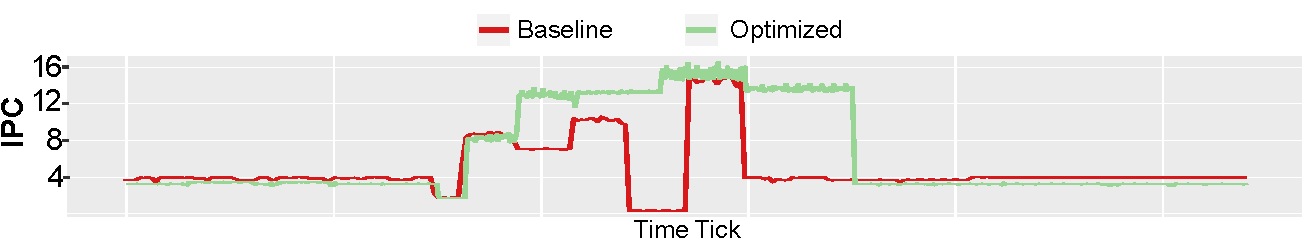
\includegraphics[width=\textwidth]{cases-paper/graphics/motivation/code_opt_3.pdf}
    \caption{Impact of loop transformations on fused cores for the Disparity benchmark.} 
    \label{fig:compmotiv}
\vspace{1em}
\end{figure}

Figure~\ref{fig:compmotiv} illustrates the impact of applying loop transformations on the \bm{Disparity} benchmark compared to a standard compiler not specifically tuned for the EDGE architecture.
In this case, the two main transformations are loop unrolling and loop interchanging.
The Figure shows the IPC performance of a 16 core composition with and without optimisations.
For example, in Listing~\ref{lst:high_ipc}, the nested loop at lines 10 to 12 has a data dependency between iterations; switching the for loop headers can get rid of the dependency.
As can be seen, the impact of these transformations can be large, leading to an 12x improvement in IPC.
Figure~\ref{fig:compmotiv} shows that the optimisations allow the core-composition to sustain a high IPC phase longer than without the optimisations.
Longer high IPC phases also means that the DMP will require less switching between core compositions, thus incurring less of a reconfiguration penalty.
However, it also demonstrates that not all of the code in a program can be optimised, as the low-IPC phases do not change.
More details about the loop transformations are given in section~\ref{sec:opt} but this example illustrates the need for careful tuning of the compiler to achieve high performance on such an architecture.

%Find some citation for this
\subsection{Knowing when and how to reconfigure the processor}

Figure~\ref{fig:disp_ex} motivates the use of runtime reconfiguration to ensure that DMP can improve the performance of single threaded applications efficiently by minimising energy consumption.
Figure~\ref{fig:compmotiv} shows how modifying loops affects the performance in terms of IPC for a core composition.
Using an API, a programmer could inform the hardware when to reconfigure by using specific functions or pragmas similar to OpenMP~\cite{openmp} or OpenCL~\cite{opencl}.
Whilst this may be a viable approach to applying runtime reconfiguration, automating the decision process is a better option.

Automating the process of reconfiguring the processor enables two advantages compared to manually determining when to reconfigure the processor.
The first advantage is that it removes the responsibility from the programmer: an automated runtime reconfiguration system can detect phases and adapt to them accordingly, using information gathered from previous traces.
Second, if ever the program is modified, this may require new profiling information to be generated to ensure that manual reconfiguration calls are correct.
If the reconfiguration is automated, then it can adapt automatically to any changes made to the source code.

\paragraph*{Summary}
This section has shown that programs exhibit phases with various amount of ILP available.
A DMP can take advantage of this property to fuse a large number of cores for the high-ILP phases and fuse a smaller number of cores when ILP drops to conserve energy.
The section also illustrated the importance of fine-tuned code transformations to achieve sustained performance and increase the potential for fusing cores.
Finally it motivates the use of automating the decision as it facilitates the utility of core composition.
The next section will study in more details the expected impact of fusion using an analytical model.

